\begin{anexosenv}

\partanexos

\chapter{Especificações do nível portfólio}\label{backlogPortfolio}

\section[Temas Estratégicos]{Temas estratégicos}

\indent \textbf{Identificador:} TE01\\
\indent \textbf{Nome:} Conhecimento e acompanhamento individual dos membros da empresa\\
\indent \textbf{Prioridade:} Alta\\
\indent \textbf{Descrição:} A empresa deseja investir no setor de gestão de pessoas a fim de melhorar o desempenho das equipes nos projetos.\\

\section[Épicos]{Épicos}

\subsection[Business]{Business}

\indent \textbf{Identificador:} EP01\\
\indent \textbf{Requisito de origem:} TE01\\
\indent \textbf{Prioridade:} Alta\\
\indent \textbf{Nome:} Informações pessoais sobre membros da empresa\\
\indent \textbf{Descrição:} Há a necessidade da diretoria de gestão de pessoas ter acesso e manipular as informações pessoais, acadêmicas, profissionais e de participação em projetos externos dos membros da Zenit para que este possa identificar experiências dos membros ativos da equipe e contatá los.\\

\indent \textbf{Identificador:} EP02\\
\indent \textbf{Requisito de origem:} TE01\\
\indent \textbf{Prioridade:} Alta\\
\indent \textbf{Nome:}  Acompanhamento do desempenho de membros da empresa\\
\indent \textbf{Descrição:} Há a necessidade da diretoria de gestão de pessoas acompanhar o desempenho dos membros, para que este possa identificar dificuldades, facilidades e motivações a fim de haver uma melhor escolha destes em projetos e reconhecer o empenho do membro em relação a empresa.\\

\indent \textbf{Identificador:} EP04\\
\indent \textbf{Requisito de origem:} TE01\\
\indent \textbf{Prioridade:} Média\\
\indent \textbf{Nome:}  Acompanhamento de atividades internas do membro\\
\indent \textbf{Descrição:} A diretoria de gestão de pessoas, desejo acompanhar as atividades dos membros internas à Zenit, para saber as atividades que eles desempenharam e poder selecionar membros mais adequados para os projetos.\\

\subsection[Enable]{Enable}

\indent \textbf{Identificador:} EP03\\
\indent \textbf{Requisitos de origem:} TE01\\
\indent \textbf{Prioridade:} Alta\\
\indent \textbf{Nome:}  Servidor para aplicação web\\
\indent \textbf{Descrição:} Um servidor para disponibilizar uma aplicação web para que os funcionários da Zenit possam acessar de qualquer dispositivo.\\


\chapter{Especificações de features}\label{backlogFeatures}

\section[EP01: Informações sobre membros da empresa]{EP01: Informações sobre membros da empresa}

\subsection[Business]{Business}

\indent \textbf{ID: FT01\\
Nome:} Gerenciar informações acadêmicas\\
\indent \textbf{Prioridade:} Altíssima\\
\indent \textbf{Descrição:} Os membros da empresa precisam inserir e manter atualizada suas informações acadêmicas, para permitir à empresa conhecê-los.\\

\indent \textbf{ID: FT02 \\
Nome:} Gerenciar informações externas a Zenit\\
\indent \textbf{Prioridade:} Altíssima\\
\indent \textbf{Descrição:} Os membros da empresa precisam inserir e manter atualizada suas informações externas a Zenit, para permitir à empresa conhecê-los.\\

\indent \textbf{ID: FT04 \\
Nome:} Gerenciar um cadastro pessoal\\
\indent \textbf{Prioridade:} Alta\\
\indent \textbf{Descrição:} Os membros da empresa precisam inserir e manter atualizada suas informações relativas aos dados pessoais, para permitir à empresa conhecê-los.\\

\subsection[Enables]{Enables}

\indent \textbf{ID: FT05\\
Nome:} Integração com módulo de projetos\\
\indent \textbf{Prioridade:} Baixa\\
\indent \textbf{Descrição:} Possuir uma interface para acesso aos dados que possibilite integração com módulo de gestão de projetos.\\

\indent \textbf{ID: FT06\\
Nome:} Controle de perfil de acesso\\
\indent \textbf{Prioridade:} Altíssima\\
\indent \textbf{Descrição:} Os funcionários que não tenham perfil de gestor só poderão acessar e modificar suas próprias informações, para garantir a integridade dos dados.\\

\section[EP02: Acompanhamento do desempenho de membros da empresa]{EP02: Acompanhamento do desempenho de membros da empresa}

\subsection[Business]{Business}

\indent \textbf{ID: FT07}\\
\indent \textbf{Nome:} Gerenciamento da evolução de perfis profissionais\\
\indent \textbf{Prioridade:} Alta\\
\indent \textbf{Descrição:} Os gestores precisam inserir o perfil profissional dos assessores para poder acompanhar a evolução do perfil deles até o ideal.\\

\indent \textbf{ID: FT08}\\
\indent \textbf{Nome:} Acompanhamento motivacional dos membros \\
\indent \textbf{Prioridade:} Alta\\
\indent \textbf{Descrição:} O gestor de pessoas quer saber o quanto os funcionários tiveram de desempenho baseados nos critérios pontuados por ele, para poder bonificar, com o prêmio escolhido pelos próprios funcionários, os que obtiveram maior desempenho.\\

\indent \textbf{ID: FT09}\\
\indent \textbf{Nome:} Suporte ao acompanhamento dos gestores \\
\indent \textbf{Prioridade:} Baixa\\
\indent \textbf{Descrição:} Os gestores da Zenit querem ter acesso as informações dos membros e poder notificar ao gestor de pessoas os membros que não estejam bem.\\

\indent \textbf{ID: FT10}\\
\indent \textbf{Nome:} Acompanhamento de presença\\
\indent \textbf{Prioridade:} Baixa\\
\indent \textbf{Descrição:} Responsável por gerenciar o quadro de horários dos membros da empresa, com a geração de um relatório de presença, a fim de identificar membros não assíduos.\\

\indent \textbf{ID: FT18}\\
\indent \textbf{Nome:} Mecanismos de busca de informações sobre os membros\\
\indent \textbf{Prioridade:} Altíssima\\
\indent \textbf{Descrição:} O gestor de pessoas precisa buscar informações sobre os membros e poder filtrá-las para facilitar o acesso a essas informações e para que se possa fazer o mapeamento das habilidades procuradas pelo gestor de pessoas nos membros\\

\section[EP03: Servidor para aplicação web]{EP03: Servidor para aplicação web}

\subsection[Enables]{Enables}

\indent \textbf{ID: FT11}\\
\indent \textbf{Nome: }Padrão arquitetural da aplicação web Model-View-Controller\\
\indent \textbf{Prioridade:} Altíssima\\
\indent \textbf{Descrição:} Uso do framework de desenvolvimento Ruby on Rails, para que a aplicação seja desenvolvida no padrão arquitetural em três camadas: model, view e controller.\\

\indent \textbf{ID: FT12}\\
\indent \textbf{Nome:} Disponibilidade do serviço\\
\indent \textbf{Prioridade:} Alta\\
\indent \textbf{Descrição:} O sistema deve estar disponível de segunda a sexta, 24 horas por dia, para que os membros possam acessar o sistema enquanto estiverem trabalhando.\\


\indent \textbf{ID: FT13}\\
\indent \textbf{Nome:} Interfaces de interação responsivas\\
\indent \textbf{Prioridade:} Alta\\
\indent \textbf{Descrição:} O sistema deve adaptar as interfaces de interação com o usuário de acordo com a resolução dos dispositivos, para que aquele possa ser acessado por dispositivos móveis e desktop.\\

\section[EP04: Acompanhamento de atividades internas do membro]{EP04: Acompanhamento de atividades internas do membro}

\subsection[Business]{Business}

\indent \textbf{ID: FT014}\\
\indent \textbf{Nome: }Gerenciamento das informações dos membros em projetos internos à Zenit\\
\indent \textbf{Prioridade:} Altíssima\\
\indent \textbf{Descrição:} Os gestores precisam inserir os dados sobre projetos internos à empresa dos membros, para que os gestores possam acompanhar melhor o desenvolvimento dos membros em projetos e selecioná-los em projetos futuros.\\

\indent \textbf{ID: FT17}\\
\indent \textbf{Nome: }Gerenciamento das Informações sobre as atividades da área interna membros na empresa\\
\indent \textbf{Prioridade:} Média\\
\indent \textbf{Descrição:} Os gestores precisam inserir as atividades delegadas aos membros da empresa, para que os gestores possam acompanhar melhor o desenvolvimento das tarefas de seus assessores.\\

\indent \textbf{ID: FT15}\\
\indent \textbf{Nome:} Gerenciamento das informações internas pessoais à Zenit\\
\indent \textbf{Prioridade:} Média\\
\indent \textbf{Descrição:} O membro precisa ter acesso a informações pessoais relativas a suas atividades internas à Zenit, para que os gestores possam ter total controle sobre as atividades do membro.\\

\indent \textbf{ID: FT16}\\
\indent \textbf{Nome:} Gerenciamento das informações sobre mini cursos\\
\indent \textbf{Prioridade:} Média\\
\indent \textbf{Descrição:} O gestor de pessoas insere os seus dados sobre participação em mini cursos oferecidos pela empresa, para que fique associe o mini curso com o membro e ele possa ser selecionado para projetos relacionados aos conteúdos aprendidos ou ministrados.\\

\chapter[Especifica{\c c}{\~o}es de Hist{\'o}rias]{Especificação de Histórias}\label{especUs}

\section{Informações pessoais sobre membros da empresa}
\subsection{Gerenciar informações acadêmicas}

\indent \textbf{Nome: Ver disciplinas cadastradas\\
    \indent Prioridade: Média\\
    \indent Identificador: US01\\
    \indent Descrição:}
    Eu, como Gestor de pessoas, quero ver todas as disciplinas cadastradas, para que eu possa gerencia-las.\\
\indent \textbf{Critérios de aceitação:}
 \begin{itemize}
            \item O gestor de pessoas deve poder ver em forma de lista, ordenada alfabeticamente, todas as disciplinas cadastradas no sistema que representará as matérias das grades das engenharias.
\end{itemize}
        

\indent \textbf{Nome: Inserir novas disciplinas\\
    \indent Prioridade: Altíssima\\
    \indent Identificador: US02\\
    \indent Descrição:} Eu, como Gestor de pessoas, quero adicionar uma disciplina, para que os membros possam adicioná-las em seu perfil acadêmico.\\
\indent \textbf{Critérios de aceitação:}
\begin{itemize}
            \item O gestor de pessoas deve poder adicionar o nome de uma disciplina em uma lista que representará todas as matérias das grades das engenharias.
            \item A informação necessária é somente: nome da disciplina. Sendo este um campo obrigatório.
            \item A ação de adicionar a disciplina pode ser cancelada.
            \item Campos obrigatórios não preenchidos devem gerar mensagem de erro ao tentar salvá-los.
            \item Os dados só são registrados ao pressionar o botão “Cadastrar disciplina”
            \item   Após a confirmação do cadastro da disciplina deve se aparecer uma mensagem com a seguinte informação: “Cadastro da disciplina efetuado com sucesso”.
\end{itemize}


\indent \textbf{Nome: Remover disciplinas\\
    \indent Prioridade: Baixa\\
    \indent Identificador: US03\\
    \indent Descrição:} Eu, como Gestor de Pessoas, desejo remover uma disciplina cadastrada, para que os membros possam adicionar apenas disciplinas existentes ao seu perfil.\\
\indent \textbf{Critérios de aceitação:}        
 \begin{itemize}
            \item Deve ter um ícone de exclusão ao lado do item da lista com o nome da disciplina que se deseja excluir, para que somente o gestor de pessoas possa remover uma disciplina cadastrada.
            \item Quando o gestor pressionar o botão de remoção da disciplina deve se gerar uma mensagem de confirmação da exclusão da disciplina com a seguinte mensagem: “Tem certeza que deseja remover esta disciplina?”. Seguida das opções: “Sim” e “Não”, em forma de botões. 
            \item Após a confirmação da exclusão da disciplina deve se aparecer uma mensagem com a seguinte informação: “Exclusão da disciplina efetuada com sucesso”.
            A ação de exclusão da disciplina pode ser cancelada.
\end{itemize}

\indent \textbf{Nome: Adicionar informações acadêmicas\\
    \indent Prioridade: Altíssima\\
    \indent Identificador: US04\\
    \indent Descrição:} Eu, como membro, quero inserir minhas informações acadêmicas para que o gestor de pessoas possa me selecionar para uma atividade ou projeto, baseado nos meus conhecimentos acadêmicos.\\
\indent \textbf{Critérios de aceitação:}        
\begin{itemize}
    \item Deve ser fornecido ao membro um formulário onde o este inserirá sua matrícula, ano de ingresso na faculdade e semestre atual, sendo estes dados campos obrigatórios.
    \item O membro deve ser capaz de poder marcar ou desmarcar na lista de disciplinas por meio de um checkbox, a opção de: Já cursei, monitoria UnB e monitoria Zenit. Sendo estas opções campos não obrigatórios.
    \item Deve haver um quadro, representando uma agenda semanal, com todos os possíveis horários de aula, sendo estes: 08-10, 10-12. 12-13, 13-14, 14-16, 16-18, 18-20 de segunda a sábado. 
    \item Após ser clicado em um horário, deverá ser possível selecionar em uma lista de disciplinas a disciplina que será cursada, representando assim sua grade atual. Sendo assim, a matéria escolhida exibida nessa agenda semanal.
    \item A ação de cadastro pode ser cancelada.
\end{itemize}

\indent \textbf{Nome: Alterar informações acadêmicas\\
    \indent Prioridade: Baixa\\
    \indent Identificador: US05\\
    \indent Descrição:} Eu, como membro, quero modificar minhas informações acadêmicas para que eu possa manter meus dados acadêmicos atualizados.\\
\indent \textbf{Critérios de aceitação:}        
\begin{itemize}
    \item Deve ser fornecido um ícone/opção na qual o membro poderá alterar o formulário que contém Matrícula e ano de ingresso e semestre de ingresso.
    \item Deve ser fornecido a opção de quando clicado na grade de matérias que estão sendo cursadas o membro poder modifica las, ou seja, deixar sem disciplina assim como escolher outra disciplina para aquele horário.
    \item A ação de modificação dos dados acadêmicos pode ser cancelada.
\end{itemize}

\indent \textbf{Nome: Informações acadêmicas no perfil\\
    \indent Prioridade: Média\\
    \indent Identificador: US06\\
    \indent Descrição:} Eu, como membro, quero ver as informações acadêmicas dos membros para que eu buscar informações com eles e indicá-los para projetos baseado nos seus conhecimentos acadêmicos.\\
\indent \textbf{Critérios de aceitação:}        
\begin{itemize}
    \item Qualquer membro deve ser capaz de ver todos os dados no perfil.
    \item As informações devem estar disposta de maneira tabular.
\end{itemize}

\subsection{Gerenciar informações pessoais}

\indent \textbf{Nome: Inserir dados pessoais\\
    \indent Prioridade: Altíssima\\
    \indent Identificador: US01\\
    \indent Descrição:} Eu, como membro da empresa, quero inserir informações relativas aos meus dados pessoais, para permitir que à empresa me conheça melhor.\\
\indent \textbf{Critérios de aceitação:}
\begin{itemize}
    \item Os campos obrigatório são: nome, email, CPF, RG.
    \item A ação de cadastro pode ser cancelada.
    \item Campos obrigatórios não preenchidos devem gerar mensagem de erro ao tentar salvá-los.
    \item A ação de cadastro pode ser cancelada.
\end{itemize}

\indent \textbf{Nome: Visualizar dados dos usuários\\
    \indent Prioridade: Alta\\
    \indent Identificador: US02\\
    \indent Descrição:} Eu, como membro, desejo visualizar os as informações pessoais de outros membros para que eu consiga ter o contato dos demais membros.\\
\indent \textbf{Critérios de aceitação:}
\begin{itemize}
    \item Os gestores poderão visualizar todo e qualquer dado de cada membro do sistema
    \item Os membros, conselho consultivo e os trainee poderão visualizar quase todos os dados de de cada usuário do sistema, menos o CPF RG.
\end{itemize}

\indent \textbf{Nome: Manter dados pessoais atualizados\\
    \indent Prioridade:  Média\\
    \indent Identificador: US03\\
    \indent Descrição:} Eu, como membro da empresa, quero manter atualizadas as informações relativas aos meus dados pessoais, para permitir que à empresa me conheça melhor.\\
\indent \textbf{Critérios de aceitação:}
\begin{itemize}
    \item Os campos obrigatório são: nome, email, CPF, RG.
    \item Os gestores devem ser capazes de modificar os dados relativos as suas informações pessoais no \item sistema de qualquer membro;
    \item A ação de cadastro pode ser cancelada.
    \item Campos obrigatórios não preenchidos devem gerar mensagem de erro ao tentar salvá-los.
    \item A ação de cadastro pode ser cancelada.
\end{itemize}

\subsection{Gerenciar informações externas a Zenit}

\indent \textbf{Nome: Visualizar perfil profissional\\
    \indent Prioridade: Baixa\\
    \indent Identificador: US07\\
    \indent Descrição: } Para que outros membros vejam os minhas informações profissionais, como membro da Zenit, eu quero disponibilizar essas informações no meu perfil profissional.\\
\indent \textbf{Critérios de aceitação:}
\begin{itemize}
    \item Informações separadas por secções: projetos, cursos, trabalhos, conhecimentos extras e workshops.
    \item   As secções que não tem dados registrados aparecerão apenas o botão para atualizar informações desta secção.
    \item É possível encurtar uma secção clicando nela.
    \item É exibido uma lista com todos os projetos contendo os atributos: nome do projeto, atividades realizadas, data de ingresso e saída.
    \item É exibido uma lista com todos os estágios e trabalhos contendo os atributos: nome da Empresa, minhas atividades, o tempo total na empresa e as datas de entrada e saída.
    \item É exibida uma lista com todos os cursos contendo os atributos: nome do curso, carga horária, se ministrou ou participou do curso, descrição.
    \item É exibida uma lista com todos os conhecimentos extras contendo os atributos: conhecimento e nível de conhecimento.
\end{itemize}

\indent \textbf{Nome: Inserir informações da área de projetos\\
    \indent Prioridade: Altíssima\\
    \indent Identificador: US02\\
    \indent Descrição:} Eu, como membro da Zenit, desejo inserir atualizadas informações de minhas participações em projetos para que a empresa tenha conhecimento de meus trabalhos.\\
\indent \textbf{Critérios de aceitação:}
\begin{itemize}
    \item Haverá um formulário onde o usuário preencherá os campos: entidade responsável pelo projeto, nome do projeto, concluído ou não, data de ingresso e saída do projeto, atividades desempenhadas no projeto, área de conhecimento, se era remunerado, projeto era PBIC ou de extensão.
    \item Ao menos uma atividade deve ser inserida.
    \item A data de saída pode ficar em branco caso o membro ainda esteja no projeto.
    \item Os campos obrigatórios nome do projeto, data de ingresso e atividades realizadas caso não preenchidos irão gerar uma mensagem de alerta.
    \item Pode ser realizada a ação de cancelar um cadastro.
\end{itemize}

\indent \textbf{Nome: Modificar informações da área de projetos\\
    \indent Prioridade: Baixissíma\\
    \indent Identificador: US08\\
    \indent Descrição:} Eu, como membro da Zenit, desejo atualizar informações de minhas participações em projetos para que a empresa tenha conhecimento de todas contribuições nos projetos.\\
\indent \textbf{Critérios de aceitação:}
\begin{itemize}
    \item Haverá um formulário com dados pré-carregados, onde o usuário preencherá os campos: entidade responsável pelo projeto, nome do projeto, concluído ou não, data de ingresso e saída do projeto, atividades desempenhadas no projeto, área de conhecimento, se era remunerado, projeto era PIBIC ou de extensão.
    \item A data de saída pode ficar em branco caso o membro ainda esteja no projeto.
    \item Os campos obrigatórios nome do projeto, data de ingresso e atividades realizadas caso não preenchidos irão gerar uma mensagem de alerta.
    \item Pode ser realizada a ação de cancelar um cadastro.
\end{itemize}

\indent \textbf{Nome: Inserir informações da área de estágios e trabalhos\\
    \indent Prioridade: Alta\\
    \indent Identificador: US03\\
    \indent Descrição:} Eu, como membro da Zenit, desejo inserir informações dos estágios e trabalhos que já trabalhei para que a empresa tenha conhecimento de meus trabalhos.\\
\indent \textbf{Critérios de aceitação:}
\begin{itemize}
    \item Haverá um formulário onde o usuário preencherá os campos: Nome da Empresa, atividades desempenhadas, data de ingresso e saída, se era remunerado.
    \item A data de saída pode ficar em branco caso ainda esteja estagiando.
    \item Os campos obrigatórios: Nome da empresa, data de ingresso e atividades desemprenhadas.
    \item Os dados são salvos ao acionar o botão salvar.
    \item Pode ser realizada a ação de cancelar.
    \item Pode adicionar e modificar o campo de atividades.
\end{itemize}

\indent \textbf{Nome: Alterar informações da área de estágios e trabalhos\\
    \indent Prioridade: Baixíssima\\
    \indent Identificador: US09\\
    \indent Descrição:} Eu, como membro da Zenit, desejo atualizadas informações dos estágios e trabalhos que já trabalhei para que a empresa tenha conhecimento de meus trabalhos.\\
\indent \textbf{Critérios de aceitação:}
\begin{itemize}
    \item Haverá um formulário com dados pré-carregados onde o usuário preencherá os campos: Nome da \item Empresa, atividades desempenhadas, data de ingresso e saída, se era remunerado.
    \item A data de saída pode ficar em branco caso ainda esteja estagiando
    \item Os campos obrigatórios: Nome da empresa, data de ingresso e atividades desemprenhadas.
    \item Os dados são salvos ao acionar o botão salvar.
    \item Pode ser realizada a ação de cancelar.
    \item Pode adicionar e modificar o campo de atividades.
\end{itemize}

\indent \textbf{Nome: Inserir informações dos cursos\\
    \indent Prioridade: Alta\\
    \indent Identificador: US04\\
    \indent Descrição:} Eu, como membro da Zenit, desejo cadastrar informações dos cursos que já participei e ministrei para que a empresa tenha conhecimento de meus trabalhos e conhecimentos.\\
\indent \textbf{Critérios de aceitação:}
\begin{itemize}
    \item Haverá um formulário onde o usuário preencherá os campos: nome do curso, data de início, carga horária, ministrou o curso ou apenas assistiu, descrição, recebeu certificado.
    \item Os campos obrigatórios: Nome do curso, tempo de duração, ministrou ou apenas assistiu, carga horária.
    \item Pode ser realizada a ação de cancelar um cadastro.
    \item Um botão deve ser acionado para aplicar as mudanças desejadas.
\end{itemize}

\indent \textbf{Nome: Atualizar as informações dos cursos\\
    \indent Prioridade:  Baixíssima\\
    \indent Identificador: US10\\
    \indent Descrição:} Eu, como membro da Zenit, desejo atualizar informações dos cursos que já participei e ministrei para que a empresa tenha conhecimento de meus trabalhos e conhecimentos\\
\indent \textbf{Critérios de aceitação:}
\begin{itemize}
    \item Haverá um formulário com dados pré-carregados onde o usuário preencherá os campos: nome do curso, data de início, carga horária, ministrou o curso ou apenas assistiu, descrição, recebeu certificado.
    \item Os campos obrigatórios: Nome do curso, tempo de duração, ministrou ou apenas assistiu, carga horária.
    \item Pode ser realizada a ação de cancelar um cadastro.
    \item Um botão deve ser acionado para aplicar as mudanças desejadas.
\end{itemize}

\indent \textbf{Nome: Inserir informações de congressos, palestras e workshops\\
    \indent Prioridade: Média\\
    \indent Identificador: US05\\
    \indent Descrição:} Eu, como membro da Zenit, desejo inserir as informações dos Congressos, palestras e workshops que já participei para que a empresa tenha conhecimento de meus trabalhos e conhecimentos.\\
\indent \textbf{Critérios de aceitação:}
\begin{itemize}
    \item Haverá um formulário onde o usuário preencherá os campos: nome, data em que foi feito, tempo de duração, assunto tratado, se recebeu certificado.
    \item Os campos obrigatórios: nome, assunto tratado e se recebeu certificado ;
    \item Pode ser realizada a ação de cancelar a atividade;
    \item Um botão deve ser acionado para aplicar as mudanças desejadas.
\end{itemize}

\indent \textbf{Nome: Atualizar informações de congressos, palestras e workshops\\
    \indent Prioridade: Baixíssima\\
    \indent Identificador: US11\\
    \indent Descrição:} Eu, como membro da Zenit, desejo modificar as informações dos Congressos, palestras e workshops que já participei para que a empresa tenha conhecimento de meus trabalhos e conhecimentos.\\
\indent \textbf{Critérios de aceitação:}
\begin{itemize}
    \item Haverá um formulário com os campos pré-carregados com os dados anteriores, onde o usuário preencherá os campos: nome, data em que foi feito, tempo de duração, assunto tratado, se recebeu certificado.
    \item Os campos obrigatórios: nome, assunto tratado e se recebeu certificado ;
    \item Pode ser realizada a ação de cancelar a atividade;
    \item Um botão deve ser acionado para aplicar as mudanças desejadas.
    
\end{itemize}

\indent \textbf{Nome: Inserir informações atualizadas da área de conhecimentos extra\\
    \indent Prioridade: Média\\
    \indent Identificador: US06\\
    \indent Descrição:} Eu, como membro da Zenit, desejo inserir as informações dos meus conhecimentos extras para que a empresa tenha conhecimento de meus conhecimentos adquiridos externamente.\\
\indent \textbf{Critérios de aceitação:}
\begin{itemize}
    \item Haverá um formulário onde o usuário preencherá os campos: conhecimento                     ( conhecimentos que podem ser uteis para a empresa em seus projetos como idiomas que domina por exemplo), Nível de conhecimento (que será escolhido entre Básico, Intermediário e Avançado)
    \item Os campos obrigatórios: conhecimento e nível de conhecimento;
    \item Pode ser realizada a ação de cancelar;
    \item Um botão deve ser acionado para aplicar as mudanças desejadas.
\end{itemize}

\indent \textbf{Nome: Atualizar informações da área de conhecimentos extra\\
    \indent Prioridade: Baixíssima\\
    \indent Identificador: US07\\
    \indent Descrição:} Eu, como membro da Zenit, desejo modificar as informações dos meus conhecimentos extras para que a empresa tenha conhecimento de meus conhecimentos adquiridos externamente \\
\indent \textbf{Critérios de aceitação:}
\begin{itemize}
    \item Haverá um formulário com informações pré-carregadas, onde o usuário preencherá os campos: conhecimento ( conhecimentos que podem ser uteis para a empresa em seus projetos como idiomas que domina por exemplo), Nível de conhecimento (que será escolhido entre Básico, Intermediário e Avançado)
    \item Os campos obrigatórios: conhecimento e nível de conhecimento;
    \item Pode ser realizada a ação de cancelar;
    \item Um botão deve ser acionado para aplicar as mudanças desejadas.
\end{itemize}

\subsection{Gerenciar perfil de acesso}

\indent \textbf{Nome: Modificar perfis dos membros\\
\indent Prioridade: Altíssima\\
\indent Identificador: US 01\\
\indent Pontuação: 03\\
\indent Descrição:} Eu, como gestor de pessoas, desejo que os membros da empresa sejam diferenciados pelo perfil para que eles possam ter permissões de acessos diferenciadas a certo conteúdos.\\
\indent \textbf{Critérios de aceitação:}
\begin{itemize}
    \item Os membros devem ser diferenciados pelo perfil de permissão de acesso(\textbf{gestor,gestor de pessoas,presidente,assessor, treinee, conselho consultivo, desligados ou excluídos (justa causa)}).
    \item Assessores e treinees tem permissão de membro no sistema.
    \item Os excluídos e os desligados não terão poder de acesso ao sistema, apenas continuaram com seus dados mantidos.
    \item Os membros terão acesso apenas ao seu próprio perfil, e ao acesso das histórias que eles sejam o ator principal.
    \item Os gestores terão acesso a tudo que o membro tem acesso mais o acesso referente das histórias que eles sejam o ator principal.
    \item O gestor de pessoa e os presidentes terão acesso máximo no sistema.
    \item Deve se ter uma página para mudar o perfil dos usuários.
\end{itemize}

\indent \textbf{Nome: Gerar novo usuário\\
\indent Prioridade: Alta\\
\indent Identificador: US02\\
\indent Pontuação: 02\\
\indent Descrição: }Eu, como gestor de pessoa, quero poder cadastrar membros no sistema para que eles possam usufruir dos recursos do software.\\
\indent \textbf{Critério de aceitação:}
\begin{itemize}
    \item Campos obrigatórios: perfil do usuário, email da Zenit.
    \item Será criado uma senha padrão.
    \item Campos obrigatórios não preenchidos devem gerar mensagem de erro ao tentar salvá-los.
    \item A ação de cadastro pode ser cancelada.
\end{itemize}


\indent \textbf{Nome: Recuperar senha\\
\indent Prioridade: Baixa\\
\indent Identificador: US03 \\
\indent Descrição: }Eu como membro, quero poder recuperar minha senha para que eu possa voltar a ter acesso ao sistema caso eu a esqueça.\\
\indent \textbf{Critério de aceitação:}
\begin{itemize}
    \item Será criado um botão de ‘Esqueci senha’.
    \item Uma modal irá aparecer na tela com um campo que receberá o e-mail ou nome completo.
    \item Na modal terá um botão de enviar
    \item Uma nova senha será enviada para o email.
\end{itemize}

\indent \textbf{Nome: Alterar senha\\
\indent Prioridade: Média\\
\indent Identificador: US04\\
\indent Pontuação: 02 \\
\indent Descrição: }Eu como membro, quero poder alterar minha senha para que eu possa escolher uma senha mais segura.\\
\indent \textbf{Critério de aceitação:}
\begin{itemize}
    \item O membro deve poder mudar sua senha para um de sua preferência.
    \item Campos obrigatórios: Senha atual, nova senha, confirmação nova senha.
    \item Campos obrigatórios não preenchidos ou preenchidos incorretamente devem gerar mensagem de erro ao tentar salvá-los.
    \item A ação de alterar senha pode ser cancelada.
\end{itemize}

\indent \textbf{Nome: Login e logout\\
\indent Prioridade: Alta\\
\indent Identificador: US05\\
\indent Pontuação: 02\\
\indent Descrição:} Eu como membro desejo inserir meus dados de login para que eu possa ter acesso ao sistema.
\indent \textbf{Critério de aceitação: }
\begin{itemize}
    \item Campo para inserir dados do login, sendo estes: Email Zenit e Senha do membro.
    \item Botão de acessar o sistema
\end{itemize}

\section{Acompanhamento de atividades internas do membro}

\subsection{Informações pessoais e internas}

\indent \textbf{Nome: Disponibilizar horários em perfil\\
\indent Prioridade: baixíssima\\
\indent Identificador: US01\\
\indent Descrição: }Eu, como membro, quero disponibilizar os horários que estarei presente no laboratório, para que possa ser feito o acompanhamento de onde estou e o que estou fazendo.\\
\indent \textbf{Critérios de aceitação:}
\begin{itemize}
    \item Um quadro disponível para inserir e ver os horários.
    \item Os tipos de horário são: presente no escritório, reuniões de projeto, semanal, gestores.
    \item Cada tipo de horário possuirá uma cor.
    \item Para alterar é preciso clicar no botão de editar.
    \item Para persistir alterações é preciso clicar no botão salvar.
    \item O quadro conterá os horários de segunda a sexta.
    \item Os horários serão de 8h até 22h.
    \item Os horários serão separados em 2h, exceto de meio dia
\end{itemize}

\indent \textbf{Nome: Disponibilizar monitorias no perfil do membro\\
\indent Prioridade: baixa\\
\indent Identificador: US2\\
\indent Descrição:} Eu, como membro, quero ver as disciplinas de monitoria de outro membro, a fim de pedir ajuda nas disciplinas que tenho dificuldade.\\
\indent \textbf{Critérios de aceitação:}
\begin{itemize}
    \item Uma listagem com as disciplinas que o membro se dispõe a dar monitoria.
    \item Deve conter o e-mail e telefone do membro que disponibiliza a monitoria.
    \item As disciplinas devem estar em ordem alfabética.
\end{itemize}

\indent \textbf{Nome: Dar punição a membro\\
\indent Prioridade: baixíssima\\
\indent Identificador: US9\\
\indent Descrição:} Eu,como gestor de pessoas, quero adicionar uma punição ao membro, para ele estar ciente de suas transgressões.\\
\indent \textbf{Critérios de aceitação:}
\begin{itemize}
    \item Deve haver um botão para adicionar punições.
    \item Deve haver seleção do tipo de punição: advertência, suspensão, desligamento, exclusão.
    \item Os tipos desligamento e exclusão devem mudar imediatamente o perfil do membro punido.
    \item A justificativa da punição é campo obrigatório.
    \item Para completar a inserção da punição é necessário clicar em salvar.
    \item Se não selecionado um tipo de punição, será colocado advertência por padrão.
    \item Deve ser gerado uma mensagem indicando se a punição foi salva, ou se houve erro ao salvar.
    \item A data em que ocorreu a punição deve ser adicionada automaticamente, ao salvá-la.
\end{itemize}

\indent \textbf{Nome: Membro ver punições\\
\indent Prioridade: média\\
\indent Identificador: US05\\
\indent Descrição: }Eu, como membro da Zenit, quero ver as punições que já recebi, para saber todas as punições que já tomei e corrigir minha conduta.\\
\indent \textbf{Critérios de aceitação:}
\begin{itemize}
    \item Membros sem punição deve aparecer uma mensagem indicando.
    \item A lista de punições deve aparecer ordenadas pela data de criação.
\end{itemize}


\section{Gerenciar informações da Zenit}
\subsection{Gerenciamento das atividades dos membros em projetos internos à Zenit}
\indent \textbf{Nome: Registrar novo um projeto\\
    \indent Prioridade:  Altíssima\\
    \indent Identificador: US01\\
    \indent Descrição:} Eu, como um gestor, quero registrar informações de um projeto, para poder associar os membros a ele.\\
\indent \textbf{Critérios de aceitação:}
\begin{itemize}
    \item As informações necessárias serão: nome do projeto, descrição resumo, gerente do projeto.
    \item A ação de registro pode ser cancelada.
    \item O nome do projeto e o gerente responsável por ele são obrigatórios.
    \item Campos obrigatórios não preenchidos devem gerar mensagem de erro ao tentar salvá-los.
    \item Os dados só são registrados ao pressionar o botão salvar.
\end{itemize}


\indent \textbf{Nome: Alterar dados do projeto\\
    \indent Prioridade: Baixa\\
    \indent Identificador: US21\\
    \indent Descrição:} Eu, como um gestor, quero modificar informações dos projetos, para poder atualizá-lo de acordo com as mudanças ao longo do tempo.\\
\indent \textbf{Critérios de aceitação:}
\begin{itemize}
    \item As informações necessárias serão: nome do projeto, descrição resumo, gerente do projeto.
    \item A ação de modificar pode ser cancelada.
    \item O nome da área e o gestor são campos obrigatórios.
    \item Campos obrigatórios não preenchidos devem gerar mensagem de erro ao tentar salvá-los.
    \item Os dados só são registrados ao pressionar o botão salvar.
    \item Os campos devem ser preenchidos com os valores já cadastrados.
\end{itemize}


\indent \textbf{Nome: Projetos no perfil do membro\\
    \indent Prioridade: Alta\\
    \indent Identificador: US02\\
    \indent Descrição:} Eu, como membro, quero que outros membros vejam os projetos que já participei em meu perfil, para que possam me contatar para me informarem sobre coisas relacionadas ao projeto.\\
\indent \textbf{Critérios de aceitação:}
\begin{itemize}
    \item Uma lista com todos os projetos ordenados pelos que sou membro ativo, e ordem alfabética.
\end{itemize}

\indent \textbf{Nome: Ver projetos da empresa\\
    \indent Prioridade: Alta\\
    \indent Identificador: US03\\
    \indent Descrição:} Eu, como membro, gostaria de ver os projetos da empresa, para poder conhecer todos os projetos que estão acontecendo e que já passaram.\\
\indent \textbf{Critérios de aceitação:}
\begin{itemize}
    \item Uma lista com todos os nomes dos projetos.
    \item A opção para visualizar apenas projetos finalizados ou ativos.
    \item Caso nenhum projeto esteja disponível para visualização, uma mensagem de alerta deve ser emitida.
    \item Os projetos devem estar em ordem \textbf{alfabética}.
\end{itemize}

\indent \textbf{Nome:  Ver membros em projetos\\
    \indent Prioridade: Média\\
    \indent Identificador: US04\\
    \indent Descrição:} Eu, como um membro, quero ver os membros associados a um projeto, a fim de encontrar os membros e contatar para passar informações relevantes.\\
\indent \textbf{Critérios de aceitação:}
\begin{itemize}
    \item Uma listagem com o nome de todos os membros que já participaram.
    \item Ver todas as atividades desempenhadas e as datas de início e término.
    \item Um botão para exibir os membros ativos ou desativos do projeto.
\end{itemize}

\indent \textbf{Nome: Associar membros a projetos\\
\indent Prioridade: Altíssima\\
\indent Identificador: US 05\\
\indent Descrição:} Eu, como gestor, quero ativar ou desativar um membro de um projeto, para saber quais membros estão trabalhando no projeto atualmente.\\
\indent \textbf{Critérios de aceitação:}
\begin{itemize}
    \item Mudar o estado de um membro dentro do projeto.
    \item Os possíveis estados são: ativo, não ativo, não participante.
    \item O membro não pode recusar seu estado em um projeto.
    \item Uma lista é gerada com todos os membros não participantes do projeto para que possa mudar seu estado.
\end{itemize}


\indent \textbf{Nome: Adicionar atividades para membros em projetos\\
\indent Prioridade: Baixa\\
\indent Identificador: US 06\\
\indent Descrição:} Eu, como gerente, quero registrar as atividades de um membro no projeto pelo qual sou responsável, para poder acompanhar o que está fazendo.\\
\indent \textbf{Critérios de aceitação:}
\begin{itemize}
    \item A atividade conterá o nome, descrição resumo, data de início, de termino, se foi concluída ou não.
    \item Todos os campos são obrigatórios e descrição resumo optativa.
    \item Mensagem de alerta é gerada para campos obrigatórios não preenchidos.
    \item Para salvar os dados, é preciso clicar no botão salvar.
    \item O registro pode ser cancelado.
\end{itemize}

\indent \textbf{Nome: Alterar atividades de um membro em projetos\\
\indent Prioridade: Baixíssima\\
\indent Identificador: US 20\\
\indent Descrição: }Eu, como gerente, quero modificar as as atividades de um membro no projeto pelo qual sou responsável, para garantir que as atividades estejam corretas mesmo se houver erro durante a criação da atividade.\\
\indent \textbf{Critérios de aceitação:}
\begin{itemize}
    \item Os dados são pré carregados nos campos do formulário.
    \item Todos os campos podem ser alterados.
    \item Os campos nome, data de início, de termino, se foi concluída ou não são obrigatórios.
    \item Descrição resumo é campo optativo.
    \item Mensagem de alerta é gerada para campos obrigatórios não preenchidos.
    \item Para salvar os dados, é preciso clicar no botão salvar.
    \item A modificação pode ser cancelada.
\end{itemize}

\subsection{Gerenciamento das informações sobre atividades da área interna}

\indent \textbf{Nome: Inserir uma nova área interna\\
\indent Prioridade: Alta\\
\indent Identificador: US12\\
\indent Descrição:} Eu, como um gestor, quero registrar informações das áreas internas da Zenit, para poder associar os membros a ela.\\
\indent \textbf{Critérios de aceitação:}
\begin{itemize}
    \item As informações necessárias serão: nome da área interna, descrição resumo, gestor da área.
    \item A ação de registro pode ser cancelada.
    \item O nome da área e o gestor são campos obrigatórios.
    \item Campos obrigatórios não preenchidos devem gerar mensagem de erro ao tentar salvá-los.
    \item Os dados só são registrados ao pressionar o botão salvar.
\end{itemize}

\indent \textbf{Nome: Alterar informações da área interna\\
\indent Prioridade: Baixa\\
\indent Identificador: US 19\\
\indent Descrição: }Eu, como um gestor, quero modificar informações das áreas internas da Zenit, para poder atualizar as informações de uma área interna de acordo com as mudanças feitas na empresa.\\
\indent \textbf{Critérios de aceitação:}
\begin{itemize}
    \item As informações necessárias serão: nome da área interna, descrição resumo, gestor da área.
    \item A ação de registro pode ser cancelada.
    \item O nome da área e o gestor são campos obrigatórios.
    \item Campos obrigatórios não preenchidos devem gerar mensagem de erro ao tentar salvá-los.
    \item Os dados só são registrados ao pressionar o botão salvar.
\end{itemize}

\indent \textbf{Nome: Ver área interna no perfil do membro\\
\indent Prioridade: Alta\\
\indent Identificador: US 13\\
\indent Descrição: }Eu, como membro, quero que outros membros vejam as áreas internas que já fui assessor em meu perfil, para que possam me contatar para me informarem sobre coisas relacionadas a essa área.\\
\indent \textbf{Critérios de aceitação:}
\begin{itemize}
    \item É exibido somente o nome da área interna que o membro está ativo.
\end{itemize}

\indent \textbf{Nome: Ver áreas internas da empresa\\
\indent Prioridade: Média\\
\indent Identificador: US 14\\
\indent Descrição: }Eu, como membro, gostaria de ver as áreas internas da Zenit, para poder conhecer todas as áreas de atividades que a empresa tem.\\
\indent \textbf{Critérios de aceitação:}
\begin{itemize}
    \item Uma lista com todas as áreas internas.
    \item Caso nenhuma área esteja disponível para visualização, uma mensagem de alerta deve ser emitida.
    \item As áreas internas serão exibidas em ordem alfabética.
\end{itemize}

\indent \textbf{Nome: Ver assessores de uma área interna\\
\indent Prioridade: Média\\
\indent Identificador: US 15\\
\indent Descrição:} Eu, como um membro, quero ver os membros de uma área interna, a fim de encontrar os membros e contatar para passar informações relevantes.\\
\indent \textbf{Critérios de aceitação:}
\begin{itemize}
    \item Uma listagem com o nome de todos os membros que já foram assessores.
    \item Ver todas as atividades desempenhadas e as datas de início e término.
    \item Um botão para exibir os assessores ativos e desativos.
\end{itemize}

\indent \textbf{Nome: Associar membros a áreas internas\\
\indent Prioridade: Alta\\
\indent Identificador: US 16\\
\indent Descrição: }Eu, como gestor, quero ativar ou desativar um assessor da minha área interna da Zenit, para indicar quais são meus assessores.\\
\indent \textbf{Critérios de aceitação:}
\begin{itemize}
    \item Mudar o estado de um membro dentro do projeto.
    \item Os possíveis estados são: ativo, não ativo, não participante.
    \item O membro não pode recusar seu estado em um projeto.
    \item Uma lista é gerada com todos os membros não participantes do projeto para que possa mudar seu estado.
\end{itemize}

\indent \textbf{Nome: Adicionar atividades aos assessores\\
\indent Prioridade: Baixa\\
\indent Identificador: US 17\\
\indent Descrição:} Eu, como gestor, quero registrar as atividades delegadas aos assessores da minha área interna, para poder acompanhar as atividades dos meus assessores.\\
\indent \textbf{Critérios de aceitação:}
\begin{itemize}
    \item A atividade conterá o nome, descrição resumo, data de início, de termino, se foi concluída ou não.
    \item Todos os campos são obrigatórios e descrição resumo optativa.
    \item Mensagem de alerta é gerada para campos obrigatórios não preenchidos.
    \item Para salvar os dados, é preciso clicar no botão salvar.
    \item O registro pode ser cancelado.
\end{itemize}

\indent \textbf{Nome: Alterar atividades dos assessores\\
\indent Prioridade: Baixíssima\\
\indent Identificador: US 11\\
\indent Descrição:} Eu, como gestor, quero modificar as atividades delegadas aos assessores da área interna, remover informações inválidas ou incorretas do sistema.\\
\indent \textbf{Critérios de aceitação:}
\begin{itemize}
    \item Os dados são pré carregados nos campos do formulário.
    \item Todos os campos podem ser alterados.
    \item Os campos nome, data de início, de termino, se foi concluída ou não são obrigatórios.
    \item Descrição resumo é campo optativo.
    \item Mensagem de alerta é gerada para campos obrigatórios não preenchidos.
    \item Para salvar os dados, é preciso clicar no botão salvar.
    \item A modificação pode ser cancelada.
\end{itemize}

\subsection{Gerenciamento das informações sobre mini cursos}

\indent \textbf{Nome: Ver participações em minicursos no perfil\\
\indent Prioridade: Média\\
\indent Identificador: US 07\\
\indent Descrição:} Eu, como membro, quero ver os minicursos que outro membro participou no seu perfil, para que ver suas participações e motivação quanto as atividades internas da empresa.\\
\indent \textbf{Critérios de aceitação:}
\begin{itemize}
    \item Todos os minicursos que ele participou serão listados.
    \item A descrição será exibida.
\end{itemize}

\indent \textbf{Nome: Ver todos minicursos\\
\indent Prioridade: Média\\
\indent Identificador: US 08\\
\indent Descrição:} Eu, como membro, desejo ver todas as informações do minicurso, para ver o quanto eles são interessantes e todos os membros que participaram.\\
\indent \textbf{Critérios de aceitação:}
\begin{itemize}
    \item As informações mostradas são: Nome, membro ministrante, participantes, descrição e a carga horária.
    \item Todos os mini cursos são exibidos em uma lista.
\end{itemize}

\indent \textbf{Nome: Inserir novo mini curso\\
\indent Prioridade: Alta\\
\indent Identificador: US 09\\
\indent Descrição: }Eu, como gestor de pessoas, quero registrar um minicurso para armazenar os cursos que são ministrados pela Zenit.\\
\indent \textbf{Critérios de aceitação:}
\begin{itemize}
    \item Os campos obrigatórios são: nome, membro ministrante, os membros participantes e a carga horária.
    \item Os campos opcionais são: descrição e o tipo interno ou externo.
    \item A operação poderá ser cancelada.
    \item Os dados só são gravados após salvar.
    \item Mensagem de alerta é gerada caso campo obrigatório esteja em branco.
    \item Os membros serão listados no qual será selecionado apenas os participantes.
\end{itemize}

\indent \textbf{Nome: Alterar informações do mini curso\\
\indent Prioridade: Baixa\\
\indent Identificador: US 10\\
\indent Descrição:} Eu, como gestor de pessoas, quero modificar um minicurso para armazenar os cursos que são ministrados pela Zenit.\\
\indent \textbf{Critérios de aceitação:}
\begin{itemize}
    \item Os campos obrigatórios são: nome, membro ministrante, os membros participantes e a carga horária.
    \item Os campos opcionais são: descrição e o tipo interno ou externo.
    \item Todos os dados podem ser alterados.
    \item A operação poderá ser cancelada.
    \item Os dados só são gravados após salvar.
    \item Mensagem de alerta é gerada caso campo obrigatório esteja em branco.
    \item Os membros serão listados no qual será selecionado apenas os participantes.
\end{itemize}

\chapter[Documento de mudanças]{Documento de mudanças}\label{docMudanca}

\section[Intodução]{Introdução}

Após a reunião 4, na qual a equipe elicitava as histórias de usuário das features de informações profissionais e projetos, que estava relacionada ao épico de informações sobre membros da empresa, a equipe notou que algumas histórias estavam se distanciando da feature ao qual pertencia, e que talvez aquela feature não se adequasse ao épico que estava inserida. Então, a equipe achou interessante abordar a organização, que até então era a atual, de forma diferente. Nesse tópico será tratado quais foram essas mudanças.\\

\subsection[O que foi acrescentado]{O que foi acrescentado}

Foram acrescentados novas funcionalidades que apresentarão os horários internos da empresa, o controle e visualização das punições dos membros e de mini cursos, e  informações sobre as monitorias internas da empresa.\\

\subsection[O que foi retirado]{O que foi retirado}

Inicialmente nada foi retirado do escopo, apenas renomeadas para melhor definir seu novo escopo e remanejado.\\

\subsection[Mudança na rastreabilidade]{Mudança na rastreabilidade}

As funcionalidades de busca dentro de cada feature do EP01, foram granularizada em uma única feature específica para busca. Essa feature foi transferida para o EP02 como mostra o quadro de rastreabilidade de antes da mudança e depois: \\

\section[Analisar riscos]{Analisar riscos}

Nesse tópico será tratado quais são os riscos e os impactos que essas mudanças ocasionará no projeto.\\

\subsection[Riscos e impactos]{Riscos e impactos}

Como o escopo do projeto aumentou e o tempo para entregar o produto final continua o mesmo, a equipe terá que desempenhar um maior esforço para aplicar as mudanças e para desenvolver as funcionalidades que tenham maior prioridade. Isso ocasionará em um aumento no custo do projeto,  provocará um possível atraso nas funcionalidades consequentes e/ou diminuirá a qualidade do produto final.\\

\section[Rastrear mudanças]{Rastrear mudanças}

Nesse tópico será localizado onde as mudanças serão aplicadas no sistema.\\

\subsection[A nível de épico]{A nível de épico}
    
As novas funcionalidades apresentadas no tópico 1.1 serão alocadas em um novo épico chamado: “acompanhamento de atividades internas do membro”(EP04).\\
    
\subsection[A nível de feature]{A nível de feature}

A antiga divisão das features “gerenciar informações de projetos” e “gerenciar informações profissionais” sofreram alterações. Essas alterações deram origem ao novo épico já mencionado no tópico 3.1 e a uma nova feature denominada: “gerenciar informações externas a Zenit”(FT02).\\
Cada funcionalidade mencionada no tópico 1.1 deu origem a uma nova feature dentro do épico “acompanhamento de atividades internas do membro”.\\
Além do acréscimo no escopo, houve mudanças também na rastreabilidade do sistema, em que foi criado uma nova feature para busca (“busca de informações sobre os membros”, FT17) que foi alocada no EP02.\\

\subsection[A nível de história]{A nível de história}

Como houve o acréscimo de novas features, novas histórias foram elicitadas com o cliente para essas novas features.\\
Além desse acréscimo, foram removidas as histórias referente a busca nas FT01, FT02  e Nas features do EP04 para que fosse criado a FT17 pudesse haver um detalhamento maior dessa funcionalidade.\\

\chapter[Visão]{Visão}\label{docVisao}

\section[Introdução]{Introdução}

Tradicionalmente os requisitos de um produto de software são representados em forma de um documento dando uma visão geral do sistema. Em metodologias ágeis, mesmo não tendo foco em documentação, um documento que representa a visão geral do produto é bem aproveitado com essa finalidade \cite{leffingwell2011}\\

Leffingwell (2011) diz que o documento de visão em metodologias ágeis geralmente respondem as seguintes perguntas:
\begin{itemize}
    \item Porque estamos desenvolvendo essa aplicação?
    \item O que essa solução particular resolve?
    \item Quem irá se beneficiar da solução proposta?
    \item Quais são as características e benefícios que ela provem?
    \item Quais são os requisitos não funcionais?
\end{itemize}

\section[Objetivos]{Objetivos}

O objetivo central do desenvolvimento desse sistema é levantar os requisitos e necessidades da gestão de pessoas da empresa júnior de aeroespacial da Universidade de Brasília do Gama, a Zenit Aerospace, para que seja possível automatizar alguns processos da empresa na área de gestão de pessoas diminuindo assim, sua atual ineficiência neste setor.\\

\section[O problema]{O problema}

\begin{table}[H]
    \centering
    \label{descricaodoprobelma}
    \caption{Descrição do problema}
    \begin{tabular}{|l|p{10cm}|}
        \hline
        \textbf{O problema da empresa é:} & Ineficiência da gestão de pessoas.\\
        \hline
        \textbf{Afeta:} & Os gestores da Zenit.\\
        \hline
        \textbf{As consequências são:} & Ineficiência de escolha de membros para os projetos e a desmotivação para realizar certas atividades dos membros.\\
        \hline
        \textbf{Uma solução bem sucedida seria:} & Um sistema que centralizaria as informações dos membros da empresa\\
        \hline
    \end{tabular}
\end{table}


O principal problema que a empresa deseja solucionar é a ineficiência na gestão de pessoas. Este problema é ocasionado por sub problemas que estão apresentados no diagrama de causa e efeito representado pela figura \ref{causaEfeito}:\\

\begin{figure}
    \centering
    \includegraphics[width=600pt,height=300pt,angle=90]{figuras/Inefici_ncia_na_gest_o_de_pessoas_p.eps}
    \caption{Diagrama de causa e efeito\label{causaEfeito}}
\end{figure}

\subsection[As subdivisões do problema]{As subdivisões do problema}


Nesse tópico será descrita as subdivisões do problema de ineficiência na gestão de pessoas.\\

\subsubsection[Motivação dos membros]{Motivação dos membros}

O departamento gestão de pessoas se preocupa com a falta de motivação dos membros, pois ela atrapalha o rendimento deles na empresa, por eles não verem reconhecimento no trabalho realizado diminuindo assim, sua proatividade e empenho na execução das tarefas.\\
Atualmente, não há nenhum processo aplicado para resolver esse problema, apenas um desenho de uma solução que ainda não é executada.\\

\subsubsection[Acompanhamento individual]{Acompanhamento individual}


O departamento gestão de pessoas empresa não consegue acompanhar as atividades internas e externas desempenhadas pelos membros dentro da própria empresa. Entende-se como atividades internas aquelas relacionadas ao desempenho delas dentro da própria empresa, atribuídas pelos gestores dos departamentos a seus assessores, assim como as dos gestores de projetos ao integrantes. Como externas, os trabalhos realizados pelos membros que não estejam associadas a empresa, tais como participações em congressos, outros projetos.\\
Apenas os próprios gestores, ao qual o membro é subordinado, conseguem acompanhar as tarefas internas dos projetos e do departamento destinadas a ele. Dessa forma, o departamento não é capaz de saber quais membros possuem um bom desempenho e atividades externas o membro tem.\\
Além disso, os gestores traçam um perfil ideal, ao qual o assessor deve seguir. Atualmente, isto é feito em papel, o que dificulta o gestor de pessoas acompanhar a evolução do perfil do membro e se este está realmente tendo alguma evolução.\\

\subsubsection[Falta de dados sobre os membros]{Falta de dados sobre os membros}

Atualmente, a empresa contém apenas os dados pessoais dos membros, tais como: número de contato, e-mail, nome, endereço, idade, entre outros, estes  considerados superficiais pelo gestor de pessoas.  Como consequência, os gestores não tem conhecimento sobre as habilidades e capacidades dos integrantes da empresa, o que dificulta o direcionamento destes para novos projetos e atividades a serem desempenhadas em nome da empresa.\\

\subsubsection[Não cumprimento de horários]{Não cumprimento de horários}


O não cumprimento de horários é ocasionado por vários fatores, entre eles a falta de motivação dos membros, a sobre carga com outras atividades fora da empresa e o monitoramento ineficiente de presença, atrapalhando assim, o desempenho dos membros nas atividades designadas a eles.\\
Atualmente a empresa tem uma lista de presença em papel, nela os membros tem que assinar seu nome todos os dias que eles trabalham sendo que ninguém monitora se isso ocorre ou não, e muitas das vezes eles esquecem de preenchê-la, com isso conclui-se que estes membros não estão cumprindo com suas obrigações.\\

\subsection[A solução]{A solução}

Esse tópico trata das soluções adotadas para cada subproblema descrito no tópico anterior, analisando os problemas que serão solucionados pelo sistema em questão.\\

\subsubsection[Motivação dos membros]{Motivação dos membros}

O gestor de pessoas tem um processo desenhado que  ajuda a entender quais as motivações dos assessores e bonifica quem cumpre com os critérios a serem definidos por ele, resolvendo em tese, todos os derivados desse problema apresentado na Figura 01. Por conseguinte, ao considerar que o problema possui uma solução completa definida por um processo, este produto o automatizará.\\

\subsubsection[Acompanhamento individual]{Acompanhamento individual}

Para que o gestores possam cumprir suas funções e acompanhar as atividades e desempenho dos membros, a solução é produzir um histórico de realizações dos membros preenchidas pelos gestores responsáveis, de forma que somente os gestores e o próprio membro tenham acesso.\\
O gestor salva um perfil ideal e o atual de um assessor e atualiza as informações de acordo com o desenvolvimento dele, mantendo um histórico para que o gestor responsável, o gestor de pessoas e o próprio integrante possam visualizar a evolução.\\

\subsubsection[Falta de dados sobre os membros]{Falta de dados sobre os membros}

Armazenar todas as informações pessoais em um banco de dados, além de adicionar as demais informações que a empresa tem interesse em conhecer sobre os seus membros.\\
A solução não determinará um processo para a atualização das informações, apenas disponibilizará que estes possam ser manipulados e armazenados em uma base de dados.\\

\subsubsection[Não cumprimento de horários]{Não cumprimento de horários}

Como o problema de não cumprimento de horário, é relacionado também a sobre carga dos alunos com o outras atividades, essa parte do problema não terá uma solução em software. Sendo assim, será tratado apenas a ineficiência na lista de presença com uma lista de presença digital cuja assinatura é feita de forma automática, gerando uma visualização gráfica da assiduidade, eliminando a parte do problema do membro esquecer de assinar ou simplesmente, algum membro assinar por outro, com possibilidade de alertar para o gesto de pessoas caso hajam muitas faltas de um membro.\\

\subsection[Beneficiados da solução]{Beneficiados da solução}

Nesse tópico será descrito todos os beneficiados do sistema e como isso ocorrerá.\\


\subsubsection[O gestor de pessoas]{O gestor de pessoas}

A solução proposta, está focada em facilitar o processo do gestor de pessoas da Zenit, proporcionando a este a automatização dessas atividades tornando-as mais eficientes e eficaz, aumentando assim, sua produtividade.\\

\subsubsection[Os gestores]{Os gestores}

Uma das caraterísticas do sistema, é o conhecimento dos assessores pelos seus gestores. O sistema possibilita ao gestor dados do perfil do membro para que este  possa traçar medidas para moldar os seus assessores de modo que seus perfis  cheguem o mais perto do perfil ideal de cada necessidade do seu gestor.\\

\subsubsection[Os assessores]{Os assessores}

Como cada gestor terá um maior domínio dos conhecimentos sobre seus assessores, sendo assim os assessores serão melhor geridos, além do que, uma das características do sistema é motivar seus membros, e os assessores serão bonificados por essa característica do sistema.\\

\subsection[Funcionalidades do produto]{Funcionalidades do produto}

As funcionalidades do produto descreverão as características e benefícios que o sistema proporcionará a quem se beneficiará dele.\\

\subsubsection[Requisitos funcionais]{Requisitos funcionais}

\textbf{Manter informações acadêmicas:} Os membros da empresa precisam inserir e manter atualizada suas informações acadêmicas, para permitir à empresa conhecê-los.\\

\textbf{Manter informações profissionais:} Os membros da empresa precisam inserir e manter atualizada suas informações profissionais, para permitir à empresa conhecê-los.\\

\textbf{Manter informações de participações em projetos:} Os membros da empresa precisam inserir e manter atualizada suas informações relativas aos projetos da faculdade e da própria Zenit, para permitir à empresa conhecê-los.\\

\textbf{Manter informações pessoais:} Os membros da empresa precisam inserir e manter atualizada suas informações relativas aos dados pessoais, para permitir à empresa conhecê-los.\\

\textbf{Gerenciamento de perfis profissionais:} Os gestores precisam inserir o perfil dos assessores para poder acompanhar a evolução do perfil deles até o ideal. Gerenciamento da evolução do perfil dos membros.\\

\textbf{Acompanhamento motivacional dos membros:} O gestor de pessoas quer saber o quanto os funcionários tiveram de desempenho baseados nos critérios pontuados por ele, para poder bonificar, com o prêmio escolhido pelos próprios funcionários, os que obtiveram maior desempenho.\\

\textbf{Suporte ao acompanhamento dos gestores:} Os gestores da Zenit querem ter acesso as informações dos membros e poder notificar ao gestor de pessoas os membros que não estejam bem.\\

\textbf{Acompanhamento de presença:} Responsável por gerenciar o quadro de horários dos membros da empresa, com a geração de um relatório de presença, a fim de identificar membros não assíduos.\\

\subsubsection[Requisitos não funcionais]{Requisitos não funcionais}

\textbf{Segurança:} Apenas usuários com privilégio de acesso de Gestor poderão visualizar informações de desempenho.\\

\textbf{Integridade:} A atualização das informações do usuário é feita pelo próprio usuário ou usuários com perfil de acesso de gestor.\\

\textbf{Portabilidade:} O serviço web deve estar disponível para funcionar tanto no Windows quanto no Linux.\\

\textbf{Design:} O sistema deve ter uma interface que permita integrar com outros módulos de sistemas a serem construídos. Uso do padrão arquitetural em três camadas: model-view-controller.\\

\textbf{Usabilidade:} O sistema deve adaptar as interfaces de interação com o usuário de acordo com a resolução dos dispositivos.\\

\textbf{Disponibilidade:} O sistema deve estar disponível de segunda a sábado, 24 horas por dia. O sistema deve estar disponível para acesso a qualquer rede.\\

\chapter[Processo geral]{Processo geral da engenharia de requisitos}

\begin{figure}
    \centering
    \includegraphics[width=500pt,height=300pt,angle=90]{figuras/processo.eps}
    \caption[Processo geral]{Processo geral da Engenharia de requisitos}
\end{figure}

\chapter[Resumo da sprint01]{Resumo da sprint01}\label{resumoSprint}

\section{Resumo da sprint}

A sprint foi realizada do dia 13/06/2016 ao dia 20/06/2016.

\begin{figure}
    \centering
    \includegraphics[width=600pt,height=300pt,angle=90]{figuras/kambamUs.eps}
    \caption[Kambam de US]{Kambam de histórias feitas ao final da sprint 01}
\end{figure}

\begin{table}
    \centering
    \begin{tabular}{|c|c|}
        \hline
        Bom & Ruim\\
        \hline
        Aprendizado em relação a linguagem & Membros não trabalharam* \\
        Aprendizado em relação as ferramentas utilizadas & Atraso de entrega \\
        & Dificuldade com a ferramenta\\
        & Dificuldade com a linguagem\\
        \hline
    \end{tabular}
\end{table}
*Membros não trabalharem foi provocado por:  membro sem notebook durante a sprint, membro com desconhecimento da linguagem e ferramentas utilizadas, entregas de outras disciplinas e não houve pareamento.

\indent Melhorias a serem feitas: trabalhar em todos os pontos ruins levantados para torna los pontos positivos, melhorar a interação dos membros e melhorar o desempenho na linguagem

\textbf{Burndown}

Devido aos fatores de terem dois membros a menos para o desenvolvimento, a equipe demorou a terminar as primeiras histórias. Visto que deve ser configurado todas as ferramentas, os plugins, dentre outros. Apesar disso, o time conseguiu produzir o código de todas as histórias planejadas, mesmo que a usabilidade da interface gráfica não tenha ficado muito correta.

\begin{figure}[H]
    \centering
    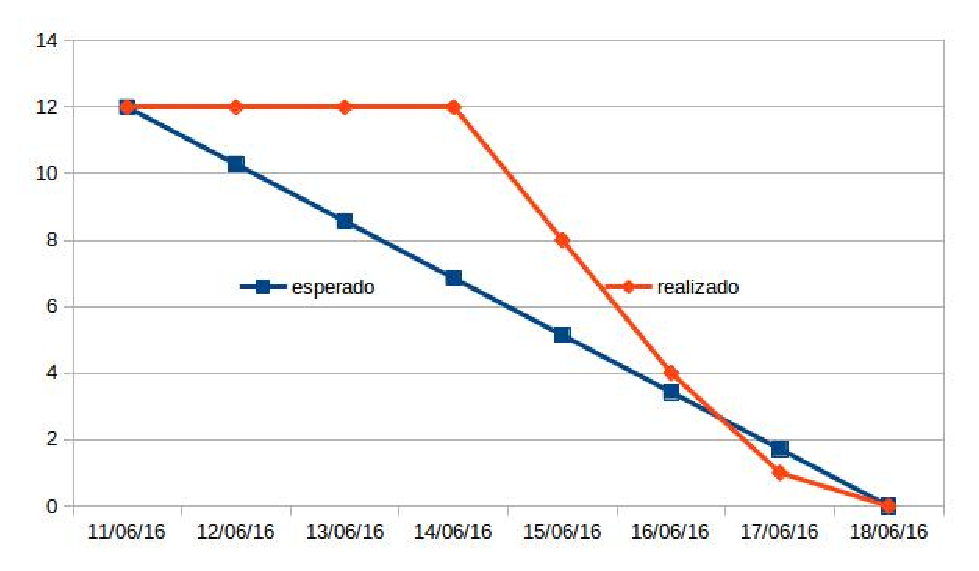
\includegraphics[keepaspectratio=true,scale=0.6]{figuras/burndown.eps}
    \caption[Burndown sprint01]{Gráfico gerado pelo burndown da sprint 01}
\end{figure}

\chapter[Entrevista para elicita{\c c}{\~a}o de temas]{Entrevista para elicitação de temas estratégicos e épicos}\label{entrevistaPortfolio}

\section{Entendendo o problema}

\begin{enumerate}
    \item Por que a sua empresa quer investir nessa área (Gestão de pessoas)?
    \newline
    \textbf{Resposta:} Melhorar a eficiência do setor de gestão de pessoas.

    \item Quais os motivos que você acha que ocasionou esse problema na gestão de pessoas?\\
    \newline
    \textbf{Resposta:} Ele, o cliente, diz que os motivos que ele pensou são: GAP de informações e não saber sobre a capacitação de seus membros.

    \item O que ocasionou o não levantamento dos dados de capacitação?\\
    \newline
    \textbf{Resposta:} Ele afirmou que houve falta de interesse, por parte dos gestores, para buscar estes tipo de informação de seus membros.

    \item E como vocês atualmente atualizam esses dados?\\
    \newline
    \textbf{Resposta:} Ele afirmou que somente os gestores tem permissão para alterar os dados obtidos, no caso só são os dados pessoais. Isso ocasiona uma sobrecarga de trabalho para os gestores por somente eles terem esse tipo de acesso.

    O Caio (Cliente), explicando sobre o processo que eles estão implementando no setor de gestão de pessoas. Comentou que alguns tópicos foram sugeridos por outras empresas juniores. Um destes foram meritocracia.

    \item Por que utilizar meritocracia?\\
    \newline
    \textbf{Resposta:} Ele afirmou que o intuito da meritocracia é motivar o membros e reconhecer esforço que eles tem em desempenhar as atividades passadas pela empresa.

    \item Como é feito o acompanhamento individual dos membros?\\
    \newline
    \textbf{Resposta:} Ele afirmou que é por meio de um questionário. Este é passado para os membros preencherem e nele tem-se algumas perguntas como: O que o motiva?. Então por meio de feedbacks diretos são feitos os acompanhamentos o individuais dos membros.
    Só o gestor de pessoas tem acesso as informações deste questionário.

    Depois passamos para entender um pouco quais são as atividades desempenhas pelo gestor de pessoas e os demais gestores.

    \item Para quem seria o sistema?\\
    \newline
    \textbf{Resposta:} Todos os gestores

    \item O que os gestores fazem?\\
    \newline
    \textbf{Resposta:} O Caio levantou algumas atividades por alto como: Manter os dados atualizados, escolher membros para projetos, fazer o acompanhamento de membros, reconhecer trabalho dos membros. Estas atividades foram completadas por um documento passado pelo Caio explicando cada atividade desempenhada por uma gestor.

    \item Uma possível solução que você imagina atualmente seria?\\
    \newline
    \textbf{Resposta:} Ele respondeu com dúvida porém posicionou se a respeito de duas opções  sendo elas: Um aplicativo para mobile ou uma aplicação WEB. 

    \item Foi questionado ao Caio, com a finalidade de visualizar mais a respeito do escopo do projeto, o que não seria contemplado na solução?\\
    \newline
    \textbf{Resposta:} Ele respondeu que não contemplaria: Gestão de projetos, Área financeira, Marketing.
\end{enumerate}

\chapter[Roadmap e Kambam de features]{Roadmap e Kambam de features}\label{rmkbft}

\section{Roadmap}

\begin{figure}[H]
    \centering
    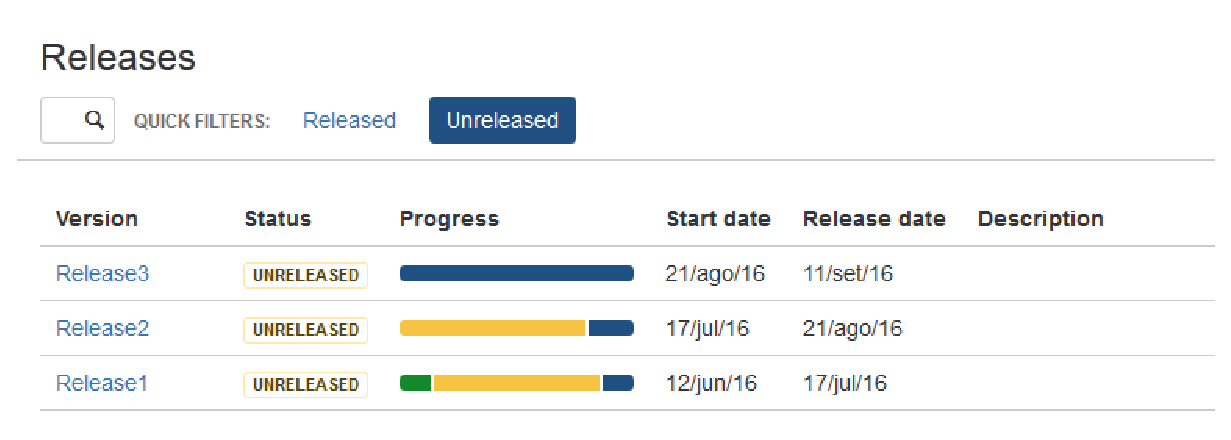
\includegraphics[keepaspectratio=true,scale=0.5]{figuras/roadmapft.eps}
    \caption[Roadmap de features]{Data de início e fim de cada uma das features}
\end{figure}

\begin{figure}[H]
    \centering
    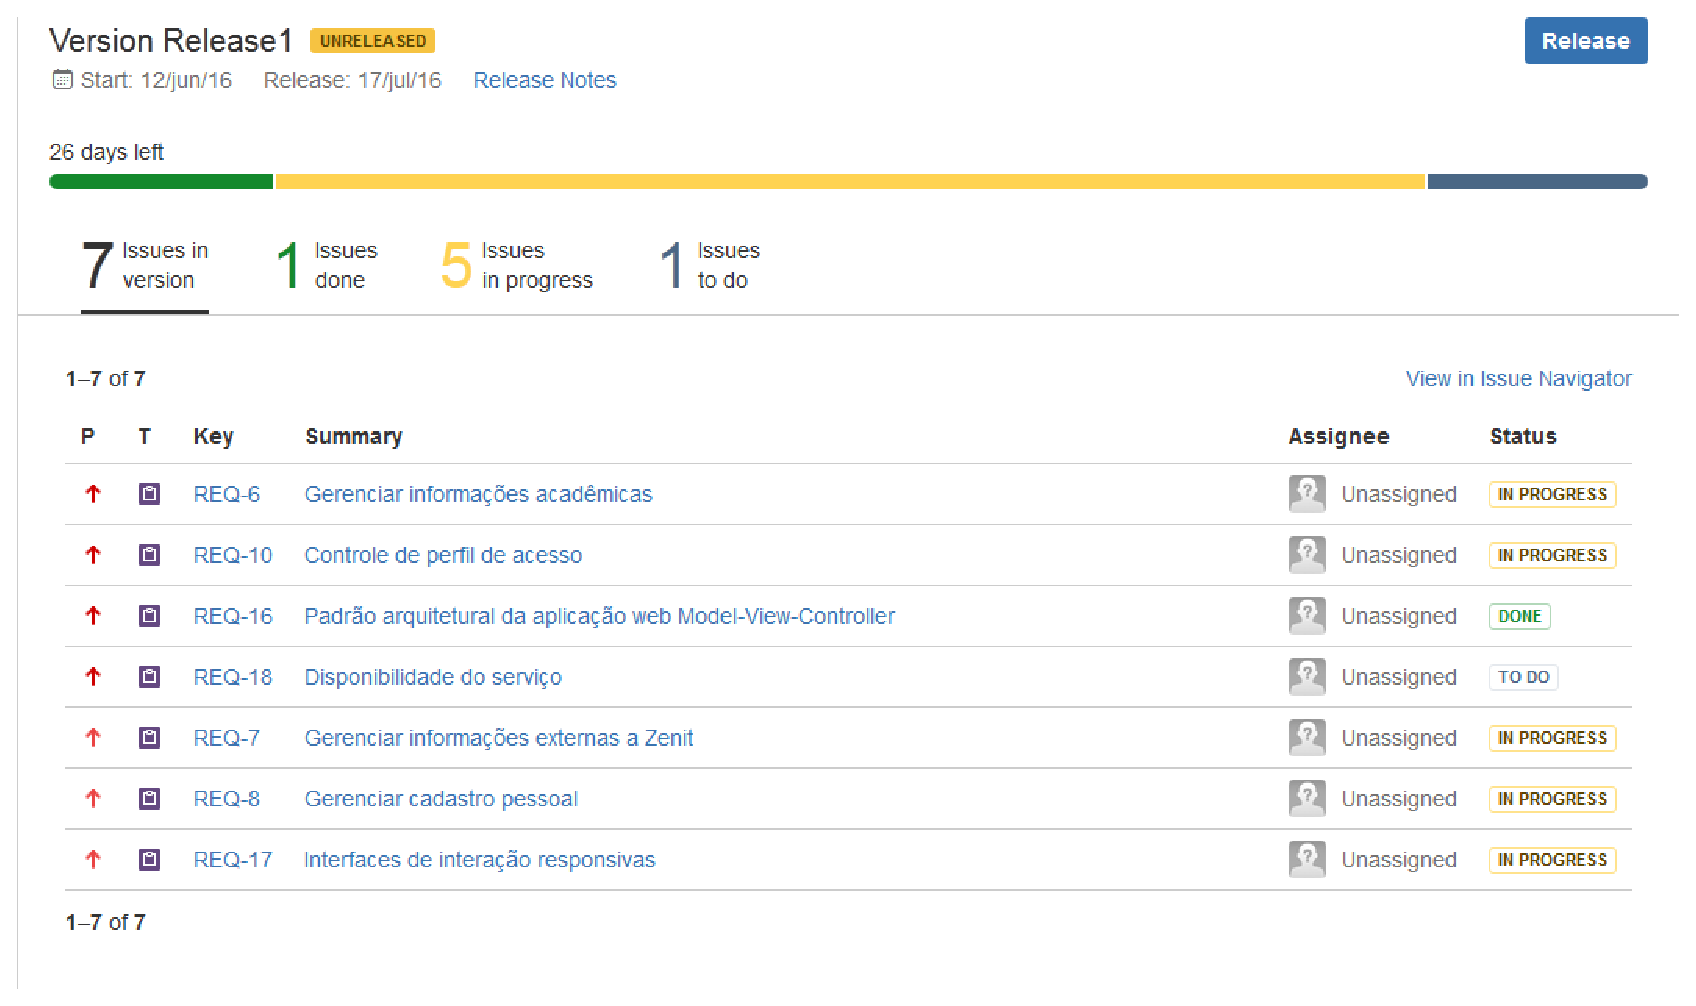
\includegraphics[keepaspectratio=true,scale=0.5]{figuras/roadmapft1.eps}
    \caption[Release 1 de features]{Features compreendidas pela release 1}
\end{figure}
\begin{figure}[H]
    \centering
    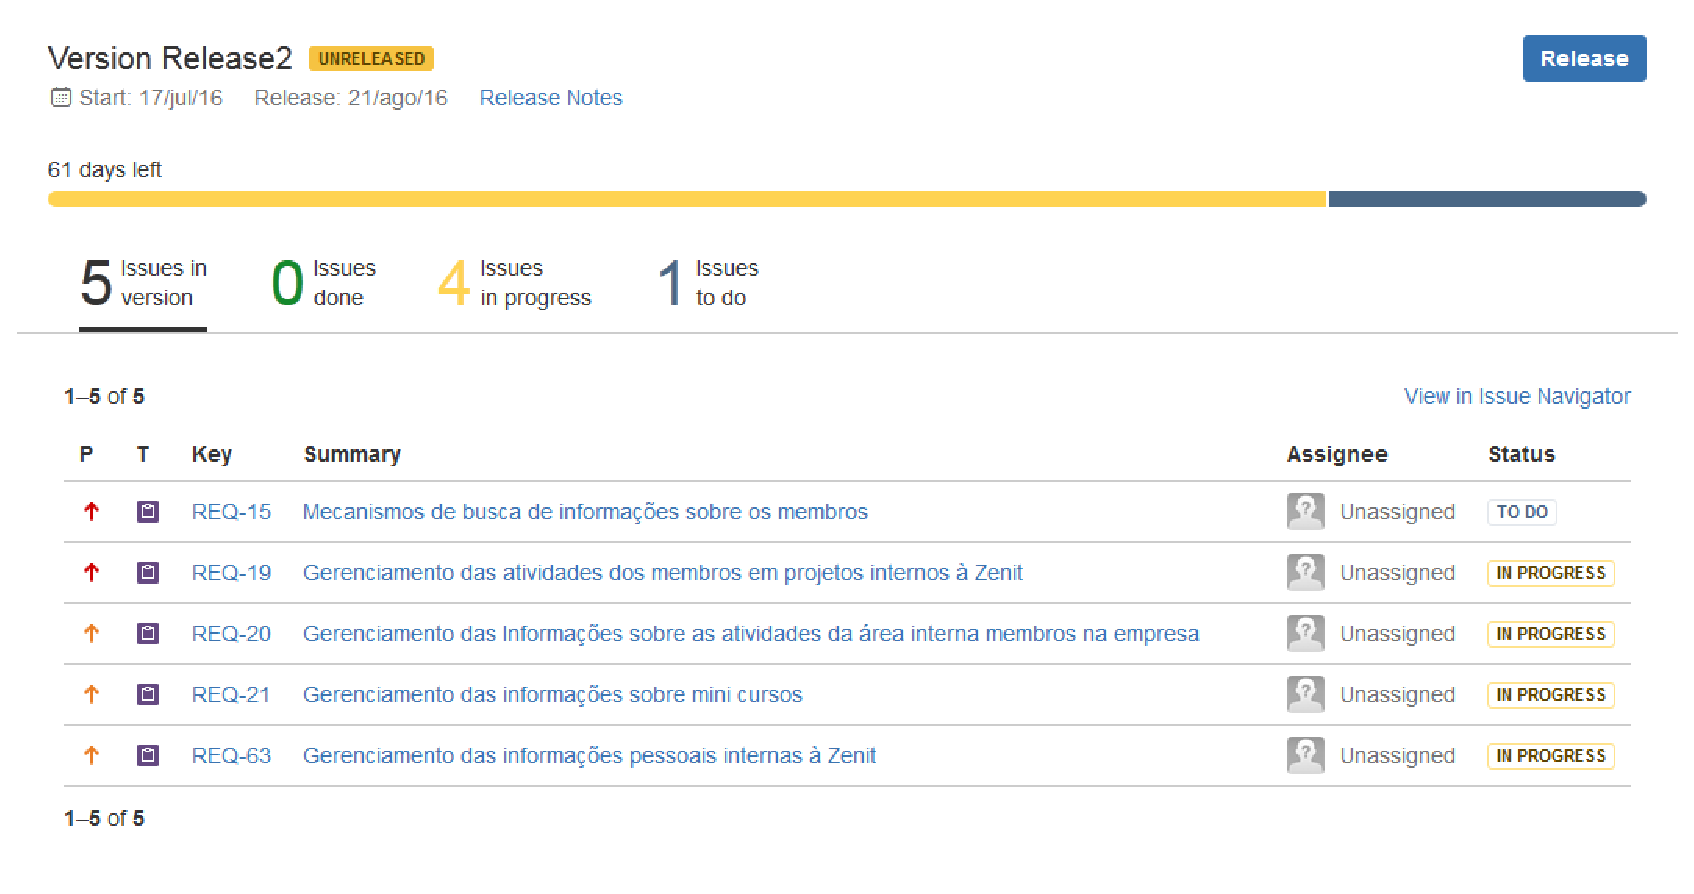
\includegraphics[keepaspectratio=true,scale=0.5]{figuras/roadmapft2.eps}
    \caption[Release 2 de features]{Features compreendidas pela release 2}
\end{figure}
\begin{figure}[H]
    \centering
    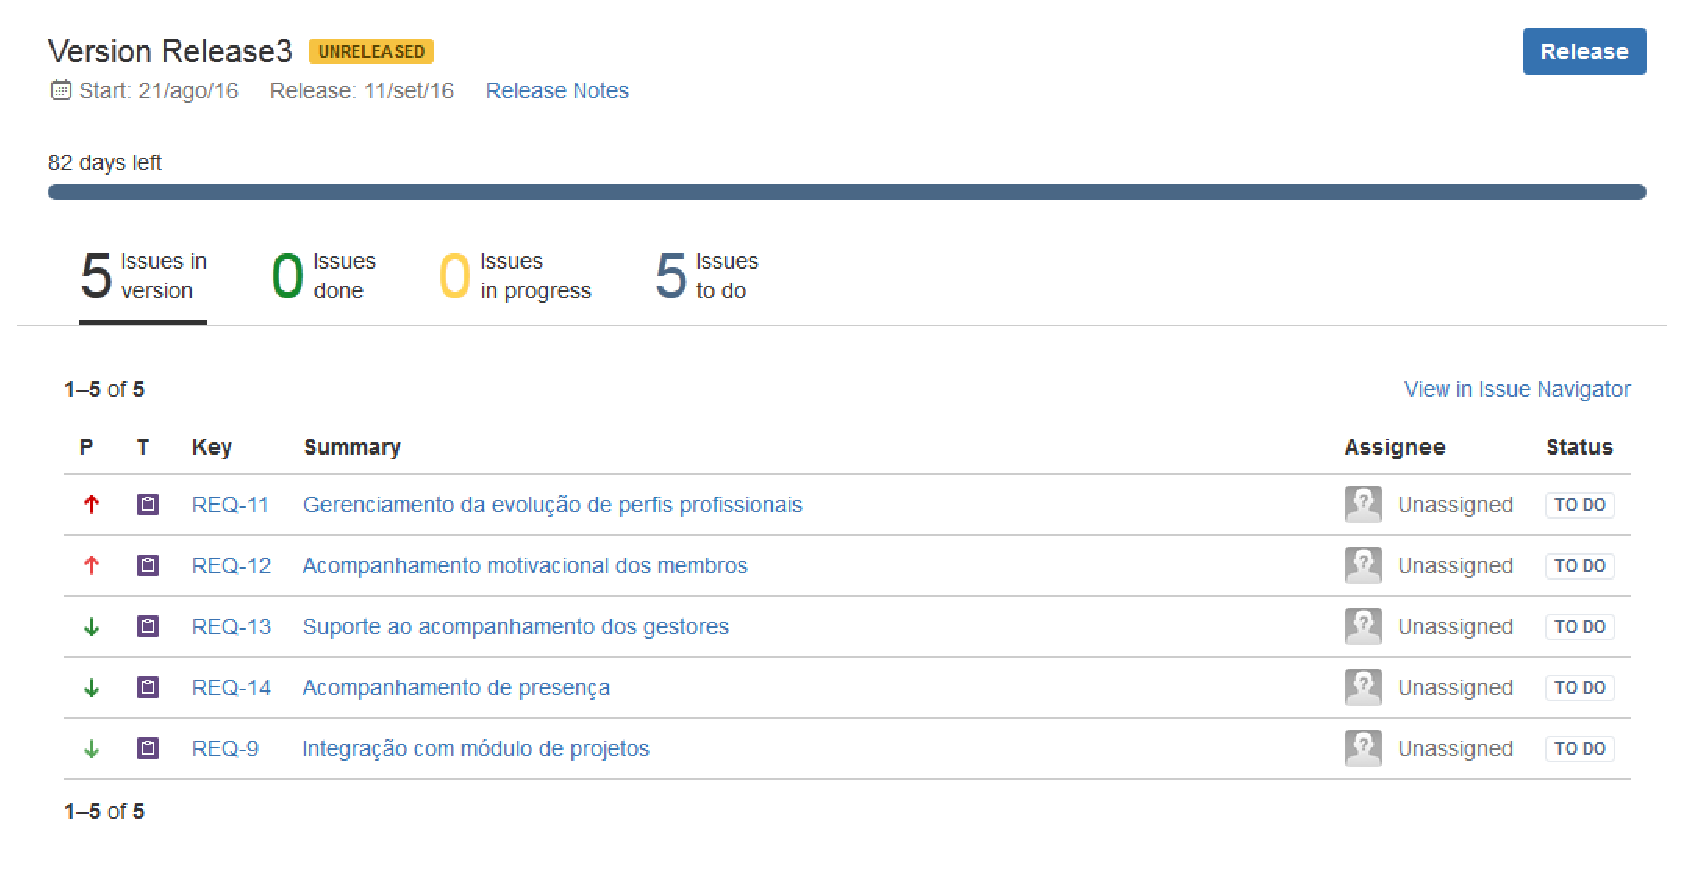
\includegraphics[keepaspectratio=true,scale=0.5]{figuras/roadmapft3.eps}
    \caption[Release 3 de features]{Features compreendidas pela release 3}
\end{figure}

\section{Kambam}

Compreende o estado atual das features. Nota-se que o estado de "doing" são para as features que foram levantadas as histórias de usuário.


\begin{figure}
    \centering
    \includegraphics[keepaspectratio=true,scale=0.5]{figuras/kambamft.eps}
    \caption[Kambam de features]{Kambam de features}
\end{figure}
\end{anexosenv}
